\FloatBarrier
\section{Historische Toninformationsträger}

\begin{figure*}[t]
    \centering
    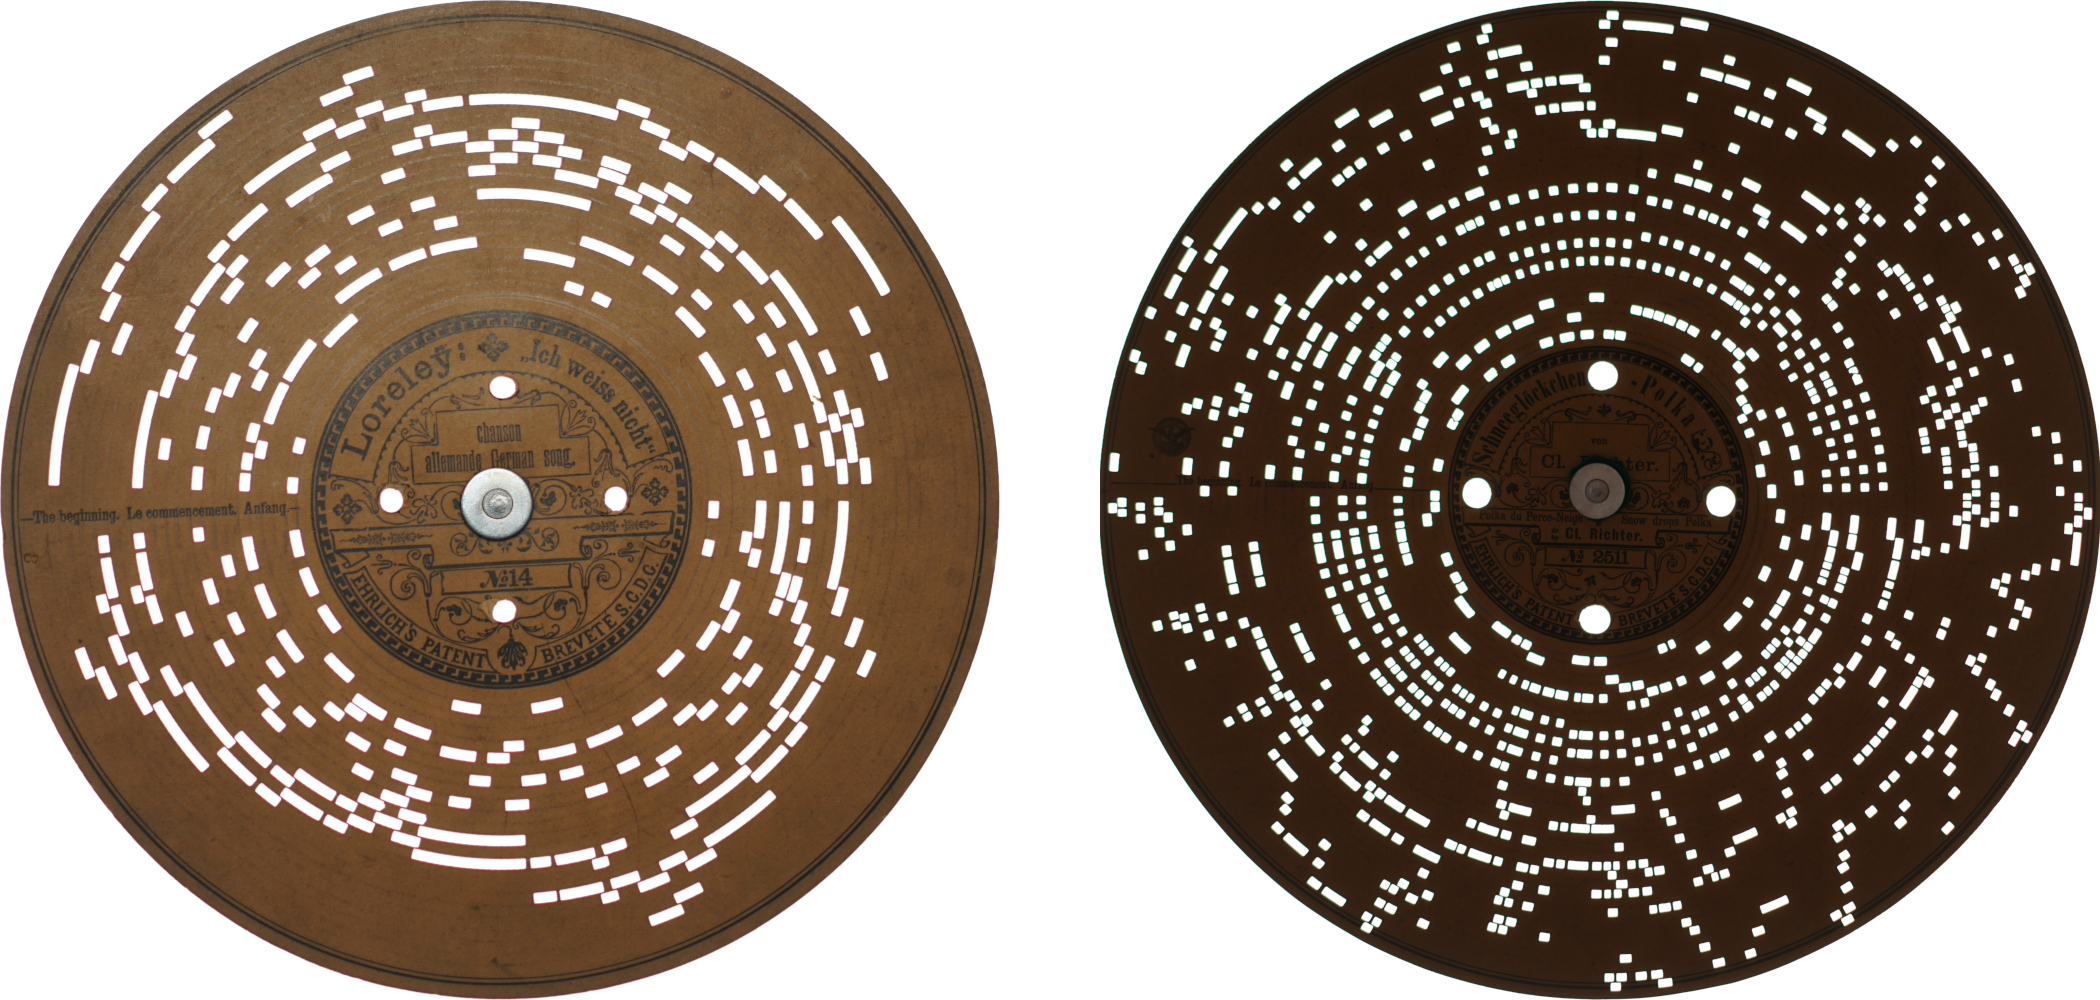
\includegraphics[width=\textwidth]{graphics/cardboard_plates.png}
    \caption{Lochplatten zweier verschiedener Formate aus dem Bestand des Musikinstrumentenmuseums der Universität Leipzig. Links eine Lochplatte des Typs Ariston, Rechts eine Lochplatte für einen mechanischen Klaviervorsetzer. Abbildungen nicht maßstabsgetreu.}
    \label{platten}
\end{figure*}

Als Toninformationsträger im Sinne dieser Arbeit werden die Medien bezeichnet, die zum Betrieb von mechanischen Musikinstrumenten benötigt werden.
Eine Definition für mechanische Musikinstrumente ist etwa in \textcite[]{mgg_mechanische} gegeben:

\begin{quotation}
    Mechanische Musikinstrumente (selbstspielende Musikinstrumente, Musikautomaten, Automatophone) sind Musikinstrumente, bei denen die Tonfolge selbsttätig durch einen Toninformationsträger gesteuert wird. Die Mehrzahl der mechanischen Musikinstrumente reproduziert Musik ohne Einwirkungsmöglichkeit des Menschen. \parencite[I. Definition]{mgg_mechanische}
\end{quotation}

Die Geschichte solcher mechanischen Musikinstrumente reicht bis in die Antike zurück, in der bereits einfache Orgeln existierten, die über das Setzen von Stiften auf einer sich drehenden Walze gesteuert werden konnten.
Den Höhepunkt ihrer Popularität erreichten die mechanischen Musikinstrumente während des späten 19. und frühen 20. Jahrhunderts, als eine Vielzahl von verschiedenen, immer komplexeren mechanischen Instrumenten konstruiert wurde \parencite[10-12]{bowers_1972}.
Mit der Entwicklung von besseren und günstigeren Methoden zur Audioaufnahme und -reproduktion um die 1930er Jahre, wurden die mechanischen Musikinstrumente praktisch komplett vom Markt verdrängt \parencite[2]{zoltan_1994}.
Für eine ausführliche Übersicht über die Geschichte der mechanischen Musikinstrumente sei auf die entsprechende Literatur verwiesen, etwa \textcite[]{bowers_1972,bowers_1975} sowie \textcite[]{mgg_mechanische}.

Die Medien für solche mechanischen Instrumente kodieren Toninformationen, mit denen das mechanische Instrument Musik erzeugen kann.
Üblicherweise werden dafür zumindest grundlegende Informationen wie der Beginn, die Länge sowie die zugehörige Tonhöhe für jeden zu spielenden Ton auf dem Medium kodiert.
Es existieren aber auch Instrumente, und mit ihnen Formate von Toninformationsträgern, die zusätzlich weitere Informationen zu Dynamik und Spielweise enthalten können.
Im Weiteren sollen vorrangig die für diese Arbeit relevanten Typen von Toninformationsträgern weiter betrachtet werden.
Diese wurden im Zeitraum zwischen 1882 und 1930 produziert und lassen sich grob in zwei Kategorien unterteilen: Plattenförmige und rollenförmige Medien.
Die plattenförmigen Medien können dabei sowohl zeitlich als auch technologisch als Vorgänger der rollenförmigen betrachtet werden können.

\subsection{Plattenförmige Toninformationsträger}

Plattenförmigen Medien wurden ab ca. 1875 produziert und stellten einen Paradigmenwechsel in der Konstruktion mechanischer Musikinstrumente dar.
Waren bei früheren Modellen die Toninformationen direkt im Instrument enthalten (beispielsweise über Walzen), wurden sie nun separat auf Platten ausgeliefert und waren somit erstmals unabhängig vom Instrument.
Eine solche Platte hat zumeist eine kurze Laufzeit von maximal einigen Minuten und konnte damit kürzere Stücke oder Motive aus größeren Kompositionen enthalten.
Durch diese Entwicklung wurde es erstmals möglich, eine größere Sammlung von Musikstücken zu besitzen \parencite[III.5.c. Plattenspieldosen und Drehinstrumente]{mgg_mechanische}.

Frühe Ausführungen dieser mechanischen Instrumente nutzten Platten aus Pappe, auf denen die Toninformationen in Form von Löchern kodiert sind, im Folgenden Lochplatten genannt.
Lochplatten dieser Formate sind sich prinzipiell recht ähnlich und unterscheiden sich vor allem in den verfügbaren Tönen, sowie den physikalischen Abmessungen der Medien.
Beispiele für zwei Lochplatten unterschiedlicher Formate dieses Typs sind in Abbildung \ref{platten} zu sehen.

Die Lochplatten sind in mehrere Spuren unterteilt, jede Spur ist einem bestimmten Ton zugeordnet.
Meist sind die Spuren aufsteigend nach Tonhöhe sortiert, mit der tiefsten Note auf der innersten Spur.
Die Töne selbst sind als Löcher binär in der Platten kodiert, dort wo ein Loch vorhanden ist klingt der Ton der entsprechenden Spur.
Anzumerken ist, dass die meisten Formate nicht chromatisch angelegt waren.
Die populären Lochplatten der Marke Ariston beispielsweise haben 24 Spuren, decken aber über 3 Oktaven ab.\footnote{Siehe \textcite[]{mxp_2003520} für eine genaue Aufschlüsselung des Tonvorrats dieses Formates.}
Durch das Auslassen bestimmter Töne ergaben sich zwar Einschränkungen bei der Kodierung von musikalischen Stücken auf die Medien, es konnte aber ein größerer Tonumfang abgebildet werden, ohne die Medien und Abspielgeräte in unpraktikable Größen zu skalieren.

\begin{figure*}[t]
    \centering
    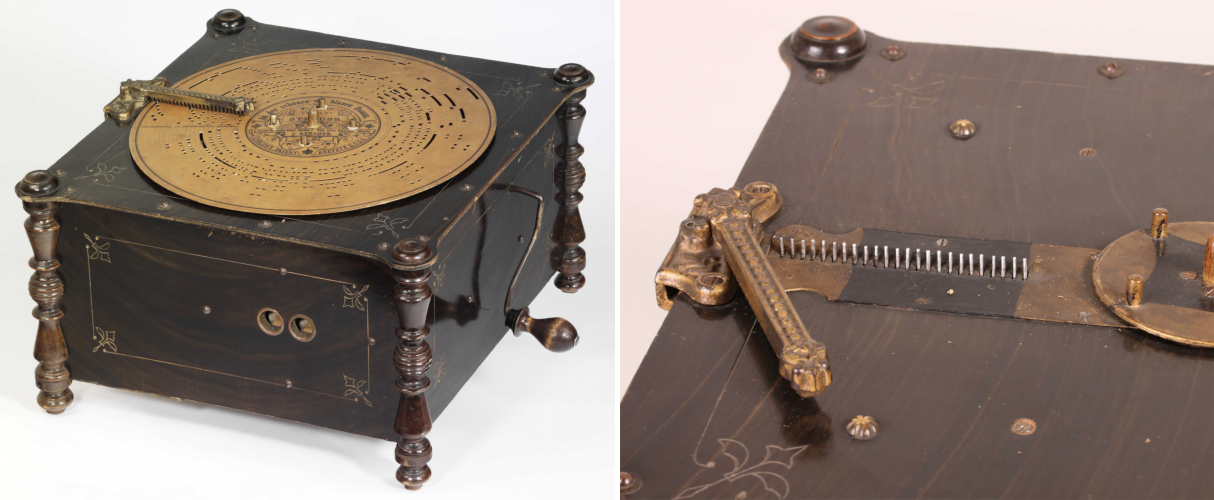
\includegraphics[width=\textwidth]{graphics/ariston_playback_device.png}
    \caption{Abspielgerät für Lochplatten der Marke Ariston aus dem Bestand des Musikinstrumentenmuseums der Universität Leipzig. Links das vollständige Gerät mit aufgelegter Lochplatte, Rechts die für die Tonerzeugung wichtige Zunge.}
    \label{aristonplayer}
\end{figure*}

Die Abspielgeräte für solche Platten (siehe Abbildung \ref{aristonplayer}) nutzen ein Verfahren zur Tonerzeugung, dass einer Mundharmonika nicht unähnlich ist.
Eine Lochplatte wird in das Abspielgerät eingelegt, das über eine Leiste mit Zungen verfügt, die den gesamten Radius des informationstragenden Teils der Lochplatte abdeckt.
Zum Abspielen wird die Lochplatte, je nach Gerät per Handkurbel oder automatisiert, gedreht und Luft wird durch die Zungen bewegt.
An den Stellen an denen Löcher vorhanden sind, kann die Luft durch die Zungen passieren, so dass ein Ton erzeugt wird.
Der so entstehende Klang dieser, auch Organetten genannten, Instrumente wurde jedoch häufig als nicht zufriedenstellend empfunden \parencite[III.5.c. Plattenspieldosen und Drehinstrumente]{mgg_mechanische}.

Eine der folgenden Entwicklungen, die gemacht wurden, um dieses Defizit im Klang auszugleichen, war der mechanische Klaviervorsetzer.
Dieser nutzt Lochplatten, die denen für die Organetten sehr ähnlich sind und Informationen nach demselben Prinzip kodierten.
Im Gegensatz zu diesen war im Abspielgerät selbst allerdings keine Tonerzeugung integriert.
Stattdessen besaß das Gerät eine Reihe mechanischer Finger, die, vor einem Klavier platziert, das auf der Lochplatte kodierte Stück auf diesem spielten.

Eine andere Weiterentwicklung der Organetten stellen plattenförmige Medien aus Metall dar.
Bei ihrer Produktion wurden kleine Teile des Blechs umgebogen, so dass Noppen entstanden, die in der Lage sind Tonkämme anzureißen.
Die Abspielgeräte für solche Platten verfügten häufig über Zusatzinstrumente wie Triangeln oder Trommeln und waren unter anderem in Wirtshäusern sehr populär \parencite[III.5.c. Plattenspieldosen und Drehinstrumente]{mgg_mechanische}.
Während die Digitalisierung solcher Metallplatten Teil des DISKOS-Projekts ist, ist sie, aufgrund der fundamental unterschiedlichen Art der Informationskodierung auf diesen Medien, kein Teil dieser Arbeit.

Im Rahmen des DISKOS-Projekts wurden Bilder eines vollständiges Konvoluts aus ca. 60 Lochplatten der Marke Ariston angefertigt, die mit der in dieser Arbeit vorgestellten Software digitalisiert werden.
Weitere ca. 40 Lochplatten für einen mechanischen Klaviervorsetzer befinden sich noch im Fotografieprozess, konnten aber bereits vereinzelt für erfolgreiche Testdigitalisierungen genutzt werden.

\subsection{Notenrollen}

\begin{figure*}[t]
    \centering
    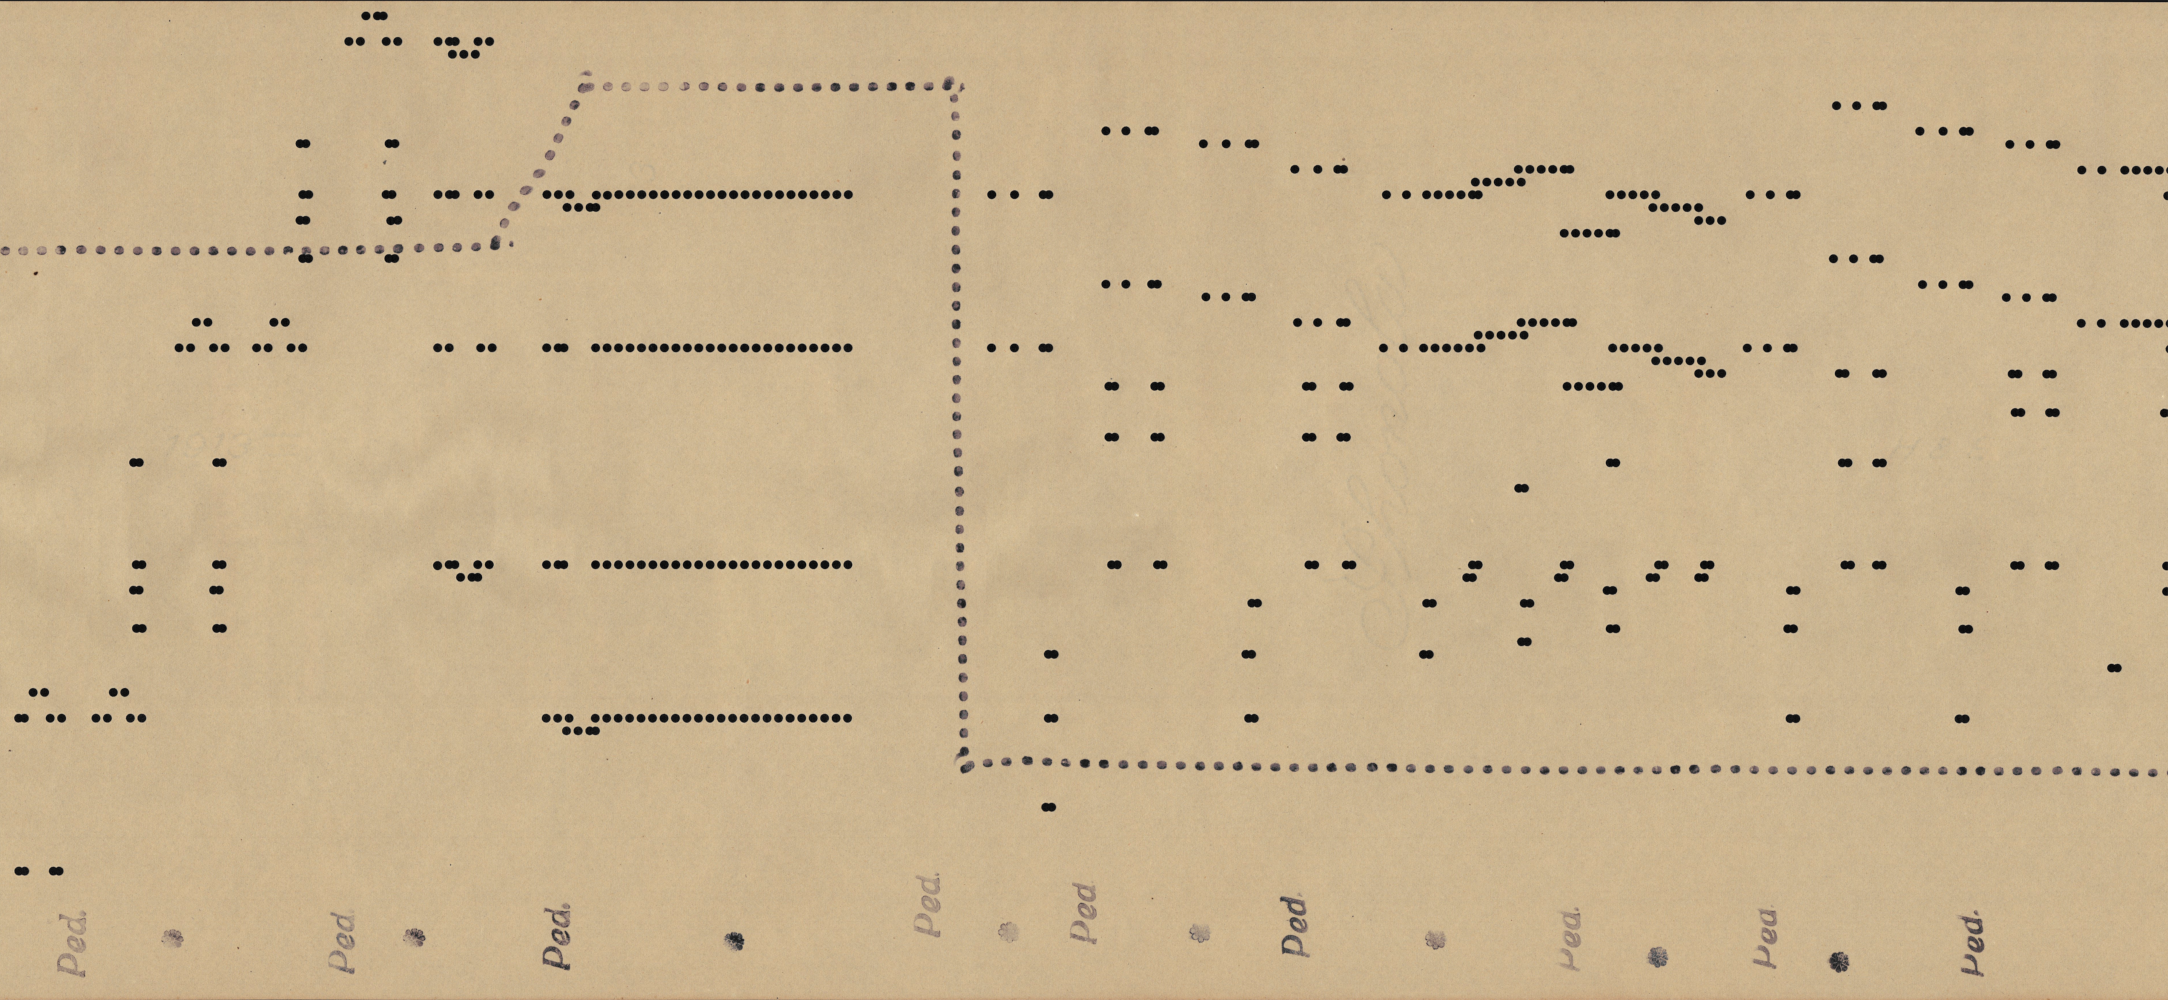
\includegraphics[width=\textwidth]{graphics/pianoroll.png}
    \caption{Abschnitt einer Notenrolle des Typs Hupfeld Phonola Solodant. Zu sehen ist neben den vorhandenen Lochungen auch eine eingezeichnete Dynamiklinie.}
    \label{pianoroll}
\end{figure*}

Während die mit der Lochplatte eingeführte Trennung zwischen Abspielgerät und Toninformationen eine signifikante Weiterentwicklung gegenüber den vorangegangenen mechanischen Musikinstrumenten darstellte, wurde mit der Notenrolle\footnote{Auch Klavierrolle genannt.} ein weiterer, wichtiger Entwicklungsschritt gemacht.
Dieses um die Jahrhundertwende eingeführte Format unterscheidet sich zum einen in der Form der Toninformationsträger, die nun als mehrere Meter lange Rollen ausgeführt wurden, aber vor allem durch die eingesetzten Techniken in den Abspielgeräten.
Ein Abschnitt einer solchen Rolle ist Abbildung \ref{pianoroll} zu entnehmen.

Die Veränderungen der Art der Informationskodierung auf Notenrollen ist im Vergleich zu Lochplatten relativ klein.
Zunächst unterscheiden sich die Notenrollen vor allem durch die neue physikalische Form als Rolle aus zumeist Papier oder Pappe, die eine Spielzeit von bis zu 15 Minuten ermöglichte.
Eine Notenrolle ist analog zu den früheren Lochplatten in mehrere Spuren unterteilt, die nun allerdings nicht mehr kreisförmig, sondern parallel, meist über die Rollenbreite von Bass (links) nach Diskant (rechts) sortiert, angelegt sind.
Die Spuren enthalten weiterhin Löcher, die über ihre Position die Toninformationen auf der Notenrolle kodieren.
Ein wesentlicher Unterschied zu Pappplatten besteht in der Kodierung länger zu spielender Töne: Diese werden nun nicht mehr durch eine durchgehende Lochung, sondern durch in sehr kurzem Abstand platzierte, sich z.T. auch überlappende, Löcher kodiert.

Frühe Abspielgeräte funktionieren, analog zu mechanischen Klaviervorsetzern für Pappplatten, als Vorsetzer und unterschieden sich im Wesentlichen durch die längere Laufzeit der Notenrollen.
Der entscheidende Vorteil dieses Systems liegt in der pneumatischen Steuerung des Abspielgeräts.
Zum Abspielen wird die Rolle in das Abspielgerät eingelegt und dieses erzeugt, bei den ersten Geräten durch menschliche Kraft, später durch Elektromotoren, ein Vakuum über die gesamte Rollenbreite.
Erreicht die Rolle nun eine Stelle, an der ein Loch vorhanden ist, kann die Luft durch das Loch strömen und so eine pneumatische Steuerung betreiben.
Diese erlaubte es über die Stärke des angelegten Vakuums auch die Stärke des Anschlags auf dem bespielten Klavier zu variieren \parencite[III.5.d. Selbstspielende Klaviere]{mgg_mechanische}.

Mit dieser Technik wurden kurz vor der Jahrhundertwende die ersten selbstspielenden Klaviere\footnote{Auch Player Pianos genannt.} konstruiert.
Die meisten dieser Klaviere verfügten über 2 separate Windladen für die Erzeugung des Vakuums und konnten so die Lautstärke von Bass und Diskant getrennt regulieren.
Während die Variation der Vakuumstärke bei den früheren Modellen, genau wie die Wahl der Geschwindigkeit, noch durch die benutzende Person erfolgte, wurden schnell zunehmend komplexere Abspielgeräte und Rollenformate entwickelt, bei denen diese Aufgaben vom Abspielgerät selbst übernommen wurde \parencite[III.5.d. Selbstspielende Klaviere]{mgg_mechanische}.

Im Jahr 1904 patentierte die Firma Welte mit dem Welte-Mignon-System das erste Reproduktionsklavier, ein System das ohne menschliche Eingaben Musikstücke wiedergeben konnte \parencite[III.5.d. Selbstspielende Klaviere]{mgg_mechanische}.
Um dies zu ermöglichen wurden Informationen beispielsweise zu Dynamik und Pedalbenutzung auf dafür vorgesehenen Spuren der Notenrolle kodiert.
Die Rollen des Typs Welte-Mignon T100 etwa, besitzen 100 Spuren von denen nur 80 zu Tönen zugeordnet sind.
Die übrigen 20 Spuren dienen zur Steuerung des Abspielgerätes \parencite[]{mxp_2002522}.

Solche Informationen konnten im Herstellungsprozess entweder manuell kodiert werden oder aber durch die direkte Aufnahme von Stücken über speziell dafür konstruierte Aufnahmeklaviere erzeugt werden.
An diesen konnten Künstler:innen ein Stück einspielen, welches danach in einem mehrstufigen Prozess durch den Rollenhersteller auf eine Masterrolle übertragen wurde.
Das genaue Verfahren mit dem dies geschah wurde durch die Hersteller mit größter Geheimhaltung geschützt und da keines der Aufnahmegeräte bis heute überdauert hat kann darüber nur spekuliert werden \parencite[]{zoltan_1994}.

Da Audioaufnahmen zur damaligen Zeit noch nicht in vergleichbarer Qualität möglich waren, bescherten grade diese eigens eingespielten Künstlerrollen den Reproduktionsklavieren eine enorme Popularität.
Schnell entwickelte sich eine Vielzahl an verschiedenen Systemen von Reproduktionsklavieren und dazugehörigen Toninformationsträgern.
In den 1920er Jahren hatte die Mehrzahl der bekannten Pianist:innen für einen oder mehrere der Hersteller Notenrollen eingespielt \parencite[]{bowers_1972}.

Im Rahmen des vorangegangenen TASTEN-Projekts wurden zwischen 2018 und 2020 am Musikinstrumentenmuseum der Universität Leipzig ca. 5000 Notenrollen in Form von Bildern digitalisiert.
Von diesen liegen ca. 3000 als vollständige Scans vor, von dem restlichen ca. 2000 Notenrollen sind nur die Anfänge der Rolle, auf denen Metainformationen wie Titel, Format, etc. vermerkt sind, gescannt worden.
Das gesamte Konvolut umfasst über 30 verschiedene Formate von Notenrollen.
Während im Rahmen des DISKOS-Projektes aus den Scans von Notenrollen aller vorliegenden Formate Midi-Dateien generiert werden sollen, beschränkt sich diese Arbeit auf Rollen des Typs Hupfeld Phonola Solodant, einem verhältnismäßig einfachen Format mit 77 Spuren.

\pagebreak